\documentclass[12pt,letterpaper]{article}

\newenvironment{proof}{\noindent{\bf Proof:}}{\qed\bigskip}

\newtheorem{theorem}{Theorem}
\newtheorem{corollary}{Corollary}
\newtheorem{lemma}{Lemma} 
\newtheorem{claim}{Claim}
\newtheorem{fact}{Fact}
\newtheorem{definition}{Definition}
\newtheorem{assumption}{Assumption}
\newtheorem{observation}{Observation}
\newtheorem{example}{Example}
\newcommand{\qed}{\rule{7pt}{7pt}}

\newcommand{\assignment}[4]{
\thispagestyle{plain} 
\newpage
\setcounter{page}{1}
\noindent
\begin{center}
\framebox{ \vbox{ \hbox to 6.28in
{\bf CS412: ntroduction to Data Mining \hfill #1}
\vspace{4mm}
\hbox to 6.28in
{\hspace{2.5in}\large\mbox{Problem Set #2}}
\vspace{4mm}
\hbox to 6.28in
{{\it Handed Out: #3 \hfill Due: #4}}
}}
\end{center}
}

\newcommand{\solution}[4]{
\thispagestyle{plain} 
\newpage
\setcounter{page}{1}
\noindent
\begin{center}
\framebox{ \vbox{ \hbox to 6.28in
{\bf CS412:   Introduction to Data Mining \hfill #4}
\vspace{4mm}
\hbox to 6.28in
{\hspace{2.5in}\large\mbox{#3}}
\vspace{4mm}
\hbox to 6.28in
{#1 \hfill {\it #2}}
}}
\end{center}
\markright{#1}
}

\newenvironment{algorithm}
{\begin{center}
\begin{tabular}{|l|}
\hline
\begin{minipage}{1in}
\begin{tabbing}
\quad\=\qquad\=\qquad\=\qquad\=\qquad\=\qquad\=\qquad\=\kill}
{\end{tabbing}
\end{minipage} \\
\hline
\end{tabular}
\end{center}}

\def\Comment#1{\textsf{\textsl{$\langle\!\langle$#1\/$\rangle\!\rangle$}}}


%\documentclass{article}
\usepackage{amsmath}
\setlength{\parindent}{0pt}
\usepackage{graphicx}
%\usepackage{fullpage}
%\usepackage{setspace} 
\usepackage{float}
%\usepackage{listings} 
%\usepackage{bbm}
\usepackage{bigstrut}
%\usepackage{caption}
%\usepackage{subcaption}
%\usepackage{algpseudocode}
%\usepackage{algorithm}

\usepackage{listings}
\usepackage{color}
\usepackage[utf8]{inputenc}

\definecolor{dkgreen}{rgb}{0,0.6,0}
\definecolor{gray}{rgb}{0.5,0.5,0.5}
\definecolor{mauve}{rgb}{0.58,0,0.82}

\lstset{frame=tb,
  language=matlab,
  aboveskip=3mm,
  belowskip=3mm,
  showstringspaces=false,
  columns=flexible,
  basicstyle={\small\ttfamily},
  numbers=none,
  numberstyle=\tiny\color{gray},
  keywordstyle=\color{blue},
  commentstyle=\color{dkgreen},
  stringstyle=\color{mauve},
  breaklines=true,
  breakatwhitespace=true,
  tabsize=3
}


\oddsidemargin 0in
\evensidemargin 0in
\textwidth 6.5in
\topmargin -0.5in
\textheight 9.0in
\usepackage{multirow}
\usepackage{hyperref}

\hypersetup{colorlinks=true}
\usepackage{color}

%\newcommand{\ans}[1]{{[{\sc Answer:} {\sf #1}]}}
\newcommand{\ans}[1]{}

\begin{document}


\solution{}{Due: 09/21/2015 11:59pm}{Assignment 1}{Fall 2015}
% Fill in the above, for example, as follows:
% \solution{Joe Smith}{\today}{1}{Fall 2012}

\pagestyle{myheadings}  % Leave this command alone

\paragraph*{General Instruction}
\begin{itemize}
\setlength{\itemsep}{2pt}
\item Errata: After the assignment is released, any further corrections of errors or clarifications will be posted at \href{https://piazza.com/class/idqujg4tiae3q0?cid=26}{the Errata page at Piazza}. Please watch it.
\item Feel free to talk to other members of the class in doing the homework. We are more concerned that
you learn how to solve the problem than that you demonstrate that you solved it entirely on your
own. You should, however, write down the solution yourself. 
\item Try to keep the solution brief
and clear. 
\item Please use Piazza first if you have questions about the homework. Also feel free to send us e-mails and come to office hours. 
\item For each question, you will \textbf{NOT} get full credit if you only give out a final result. Necessary calculation steps and reasoning are required. 

\end{itemize}

\paragraph*{Assignment Submission}
\begin{itemize}
\setlength{\itemsep}{2pt}
\item Please submit your work before the due time. \textbf{We do NOT accept late homework!}
\item {We will be using Compass for collecting the homework assignments}. Please submit your answers via Compass (\url{http://compass2g.illinois.edu}). Please do NOT hand in a hard copy of your write-up. Contact the TAs if you are having technical difficulties in submitting the assignment.
\item \textcolor{red}{The homework \textbf{MUST} be submitted in \textbf{pdf} format}. \textbf{Scanned handwritten and hand-drawn pictures} inside your documents \textbf{are not acceptable}. Answers to the written part and mini-MP should be included in one \texttt{.pdf}  file.
\item Please \textbf{DO NOT} zip the PDF file so that graders can access your PDF directly on Compass.  You can compress other files into a single zip file. In summary, you need to submit one PDF file, named as \texttt{hw1.netid.pdf}, and one \texttt{.zip} file, named as \texttt{hw1.netid.zip}.
\item If scripts are used to solve problems, you are required to submit the source code, and use the file names to identify the corresponding questions or sub-questions. For instance, \texttt{question1.netid.py} refers to the python source code for Question 1; and \texttt{question1a.netid.py} refers to the python source code for sub-question 1(a); replace \texttt{netid} with your netid. You can submit separate files for sub-questions or a single file for the entire question. 

\end{itemize}

%\paragraph*{Dataset}
%\begin{itemize}
%\item The data for Q2 can be download from compass2g or \href{http://goo.gl/0l4XkG}{the link}.    
%\end{itemize}

\paragraph*{Dataset}
\begin{itemize}
\item The data set file, data.zip, can found in  \href{https://wiki.cites.illinois.edu/wiki/display/cs412fa15/Assignments}{the course website}.    
\end{itemize}

\pagebreak

\section*{Question 1 (15 points)}
The dataset \texttt{data.online.scores} (in \texttt{data.zip}) provides the exam score records  for students who take online courses. These records are sampled from a general population. Data in each row are separated by tabs. The first column shows students' IDs. The second column is students' midterm scores and the third column is students' final scores.  Please give the following statistical descriptions of the \textbf{final scores}. If the result is not integer, then round it to 3 decimal places.\\

\textbf{Purpose} 
\begin{itemize}
\item Have a better understanding of basic statistical descriptions of data.
\end{itemize}

\textbf{Requirements} 
\begin{itemize}
\item For sub-questions (a), (b) and (c), you should write scripts to calculate statistical descriptions. There is no restrictions on the language you use. You are not allowed to calculate using calculators or by hands. You are required to submit your source code for sub-questions (a), (b) and (c).
\item For sub-question (d), you are required to answer the question in the PDF file you will submit.
\end{itemize}
\begin{itemize}
 \item[a.] (6') First quantile $Q_1$, the median, and the third quantile $Q_3$.
 \item[b.] (3') Mean.
 \item[c.] (3') Mode.
 \item[d.] (3') For the distribution of students' final scores, is the data positively skewed or negatively skewed? Explain why you could get your conclusion.
 \end{itemize}
 

\section*{Question 2 (15 points)}

In the following questions, you are required to evaluate the similarity/dissimilarity among data samples. If the result is not integer, then round it to 3 decimal places.\\

\textbf{Purpose} \begin{itemize}
\item Have a better understanding of measuring data similarity and dissimilarity.
\end{itemize} 
\textbf{Requirements} 
\begin{itemize}
\item For sub-questions (a) and (b), you should write important steps and the result in the PDF file you will submit. Only giving a result will not get credits.
\item For sub-question (c), you should explain clearly in the PDF file. \item For sub-question (d), you should write a script to calculate. There's no restrictions on the language you use. You are required to submit your source code for sub-question (d). 
\end{itemize}
 
 \begin{itemize}
 \item[a.](3') Given two objects \textit{Obj1} and \textit{Obj2}, each of them has 200 binary attributes. Table \ref{contin} is the contingency table for these two objects. Each cell in the table shows the number of attributes where \textit{Obj 1} and \textit{Obj 2} have the corresponding combination of values. E,g., for cell \textit{Obj 1} = 1 and \textit{Obj2} = 0, there are 28 attributes with such a combination. Suppose  all the attributes are \textbf{asymmetric} binary attributes, you are required to calculate the Jaccard coefficient of \textit{Obj1} and \textit{Obj2}.

\begin{table}[h]
\centering

\begin{tabular}{llll}
                                                  & \multicolumn{3}{c}{{\it Obj 2}}                                             \\ \cline{2-4} 
\multicolumn{1}{l|}{\multirow{3}{*}{{\it Obj 1}}} & \multicolumn{1}{l|}{}  & \multicolumn{1}{l|}{1}  & \multicolumn{1}{l|}{0}   \\ \cline{2-4} 
\multicolumn{1}{l|}{}                             & \multicolumn{1}{l|}{1} & \multicolumn{1}{l|}{21} & \multicolumn{1}{l|}{28}  \\ \cline{2-4} 
\multicolumn{1}{l|}{}                             & \multicolumn{1}{l|}{0} & \multicolumn{1}{l|}{39} & \multicolumn{1}{l|}{112} \\ \cline{2-4} 
\end{tabular}
\caption{Contingency Table for \textit{Obj1} and \textit{Obj 2}}
\label{contin}
\end{table}


\item[b.](6') Given two points in the 3-D space, $A = (3,1,2)$ and $B = (-1,0,8)$. Please calculate the following distances between these two points.
 \begin{itemize}
 \item[1.] \textit{Euclidean} distance.
 \item[2.] \textit{Manhattan} distance.
 \item[3.]\textit{Minkowski} distance where $h = \infty$.
 \end{itemize} 
 \item[c.] (2') Suppose we have two random points $A$ and $B$ in space, explain why the \textit{Euclidean} distance between $A$ and $B$ is always shorter than (or equal to) the \textit{Manhattan} distance?
 \item[d.] (4') Given the dataset \texttt{vectors.txt}, you will find two vectors ($A$ and $B$). Each vector has 100 attributes (separated by tabs). Calculate the following distance between these two vectors:
  \begin{itemize}
  \item[1.] \textit{Minkowski} distance where $h = 2$.
  \item[2.] \textit{Minkowski} distance where $h = 3$.
  \end{itemize}
 \end{itemize}

\section*{Question 3 (10 points)}
Based on the data of students' scores (file \texttt{data.online.scores}, contained in the file \texttt{data.zip}), normalize the mid-term scores using z-score normalization (use \textbf{empirical standard deviation} for standard deviation).\\

\textbf{Purpose} 
\begin{itemize}
\item Understand the intuition and usage of z-score normalization.
\end{itemize}

\textbf{Requirements}
\begin{itemize}
\item Write a script to normalize the data using z-score normalization, in any language of your choice. You need to include the script file in your submission.
\end{itemize}

\begin{itemize}
\item[a.] (5') Compare the mean and empirical variance before and after normalization.
\item[b.] (5') For original score of $90$, what is the corresponding score after normalization?
\end{itemize}

\section*{Question 4 (30 points)}
\textbf{Purpose}
\begin{itemize}
\item Understand the intuition and usage of Pearson correlation coefficients and Principal Component Analysis (PCA).
\end{itemize}

\textbf{Requirement}
\begin{itemize}
\item Apply the algorithms described in the lecture slides on a toy dataset
\item Give explanations based on your understanding of the algorithms
\item Use Matlab, MS Excel, or similar software applications for calculation and visualization.
\end{itemize}

Consider 10 data points in 2-D space as specified in the table below. 
\begin{table}[htb]
\begin{center}
\begin{tabular}{|c|c|c|c|c|c|c|c|c|c|c|} \hline
 $X$ & 0.69 & -1.31 & 0.39 & 0.05 & 1.29 & 0.49 & 0.19 & -0.81 & -0.31 & 0.71  \\ \hline 
 $Y$ & 0.89 & -1.11 & 0.59 & 0.45 & 1.19 & 0.69 & 0.25 & -0.71 & -0.21 & 0.71  \\ \hline
\end{tabular}
\end{center}
\end{table}
\begin{enumerate}
  \item[a.] $(5')$ What is the (Pearson) correlation coefficient between $X$ and $Y$ in the data set above? Show your calculations. What do you learn about the data set from the quantity? 

  \item[b.] $(3')$ Based on the quantity and conclusion above, without actually applying PCA, can you guess if PCA may or may not help to reduce the data size? Explain your guess by the intuition of PCA.

  \item[c.] $(6')$ What is the covariance matrix for the data set above? Show your calculation. \textit{Hint: It is easy to miss a few steps. Follow the steps described in the lecture slides.}
  
  \item[d.] $(6')$ How many principal components does the dataset have? What are they? What is the first principal component, i.e., the most important one? Show your calculation. \textit{Hint: You can use Matlab or similar software applications to find eigenvectors.}
  
  \item[e.] $(5')$ Scatterplot all the data points and draw the lines showing the directions of all the principal components. \textit{Hint: You may use Matlab or Excel to draw.}
  
  \item[f.] $(5')$ Suppose we only use the first principal component, i.e., the most important component, as the basis for the new space. Project the data points $A=(0.05, 0.45)$ and $B=(0.49, 0.69)$ to the new space. Show your calculation. Draw the projections on the figure in sub-question (e).
  
  %\controlprint{\bigv}

\end{enumerate}
\section*{Mini Machine Problem 1 (15 points)}
This MP borrows a quite considerable amount of material from a certain source. We will publish the source after the submission’s due date because it contains answers for a few questions. Don’t try to find the existing answers because the MP is not hard, and it is really fun and useful. To finish the MP, please read this document carefully.\\
In this MP, we use the Matlab  built-in data set \textbf{carsmall}, a data set containing information for 100 cars in 1970, 1976 and 1982. For this data set, we focus on 5 attributes: \texttt{Acceleration} (the rate of change of velocity of a car), \texttt{MPG} (Miles Per Gallon, fuel efficiency), \texttt{Displacement} (the volume of the cylinder), \texttt{Horsepower} and \texttt{Weight}. We use the \texttt{Cylinders} attribute (the number of cylinders) to group our observation. You will be required to run some code provided to you in this PDF file. \textbf{However, do not copy the code from this file to Matlab directly since the encoding mechanism for some special symbol in PDF is not supported by Matlab. You should type the code into Matlab.}\\

\textbf{Purpose} 
\begin{itemize}
\item Learn the basic techniques for data visualization using Matlab.
\end{itemize}
\textbf{Requirements} 
\begin{itemize}
\item This MP requires Matlab. \textit{Please do not use other softwares since that will make the assignment harder for some questions.} The software is free for UIUC students in UIUC Webstore. And it is also available in EWS machines on campus. If you are not able to access both sources, please let us know ASAP. Please also note that it may take you only 1-2 hours to finish the MP, so if you don’t often use the heavy Matlab software, you may want to use one of the EWS machines on campus.
\item You should write all your answers (code, graphs and texts) in the PDF file you will submit. For code and graphs, you could paste them to the file.  
\end{itemize}
 

\begin{enumerate}
\item[1.] Load the data \textbf{carsmall} in Matlab using the following code.
\begin{lstlisting}
load carsmall
X = [MPG,Acceleration,Displacement,Weight,Horsepower];
varNames = {'MPG'; 'Acceleration'; 'Displacement'; 'Weight'; 'Horsepower'};
\end{lstlisting}
\item[2.] (2') Comet graph is an animated graph. To trace the data points on the screen for the \texttt{Displacement} attribute, we use the following code to visualize the \texttt{Displacement} attribute. Show the \textbf{final comet graph} in the PDF file you will submit by running the following code on Matlab.
\begin{lstlisting}
comet(Displacement)
xlabel('Index of Car')
ylabel('Displacement')
\end{lstlisting}

\item[3.] (5') Drawing boxlpot is a popular way to visualize a distribution. The two whiskers show the Min observation and the Max observation. The central line shows the median. The edges of the box are the first quantile and the third quantile. 
\begin{itemize}
\item[a.] (1') Run the following code on your Matlab to draw a boxplot for the \texttt{Acceleration} attribute. Show the \textbf{boxplot}  in the PDF file you will submit.
\begin{lstlisting}
boxplot(Acceleration)
ylabel('Acceleration')
\end{lstlisting}
\item[b.] (4') Write code to visualize the \texttt{Acceleration} attribute using the boxplot for cars with different number of cylinders. In this graph, you group cars using the \texttt{Cylinders} attribute (the number of cylinders). For each group of cars, you draw a box to show the five-number summaries on \texttt{Acceleration}.  All the boxes should be drawn on the same graph. In your graph, $x$-axis represents the number of cylinders and the $y$-axis shows the \texttt{Acceleration}. You should also add the label for $x$-axis (\texttt{Cylinders}) and $y$-axis (\texttt{Acceleration}). (\textit{Hint: only several lines of codes are needed to finish this task. Try to use the boxplot(X,G) function where X is the attribute to be visualized and G is the grouping attribute.})
Show your \textbf{code and grouping boxplot} in the PDF file you will submit. 
\end{itemize}

\item[4.] (4') 3-D scatter plots are popularly used to visualize 3 attributes at the same time. 
\begin{itemize}
\item[a.] (2') Run the following code to draw a 3-D scatter plot. Show the \textbf{3-D plot} in the PDF file you will submit. 
\begin{lstlisting}
scatter3(Displacement,Cylinders,Horsepower,'filled','r')
xlabel('Displacement')
ylabel('Cylinders')
zlabel('Horsepower')
\end{lstlisting}
\item[b.] (2') By observing the graph you get, could you identify a pair of correlated attributes? Could you explain why the positive or negative correlation makes sense? Give your \textbf{answer} in the PDF file you will submit. (\textit{Hint: You could rotate the graph in Matlab when you try to find the correlation between two attributes on a 3-D graph.})
\end{itemize}

\item[5.] (4') Interactive star plots are used to show the values of attributes for each observation. In each star (observation), the spoke length is proportional to the value of that attribute for that observation.
\begin{itemize}
\item[a.] (2') Run the following code. Show the \textbf{graph} in PDF file you will submit.
\begin{lstlisting}
h = glyphplot(X(1:9,:), 'glyph','star', 'varLabels',varNames,...
'obslabels',Model(1:9,:));
set(h(:,3),'FontSize',8);
\end{lstlisting}
\item[b.] (2') In the Matlab figure dialog menu, there is a button called \textbf{data cursor} (See Figure \ref{fig:datacuror}. The data cursor item is in the red circle.) Based on the graph you get in 5a, if you click on the data cursor button, and then click on any star (car), you will get the value for each attribute of that car. Show the \textbf{value} of each attribute for the star (car) at the top left corner of the graph you plotted in the Question 5a in the PDF file you will submit.
\begin{figure}[!h]
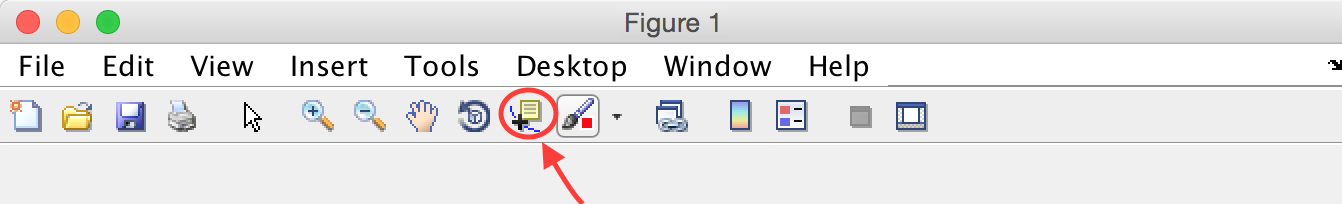
\includegraphics[width=0.5\textwidth]{pics/datacursor.png}
\centering
\caption{Matlab Figure Dialog Menu}
\label{fig:datacuror}
\end{figure}
\end{itemize}

\end{enumerate}
\section*{Mini Machine Problem 2 (15 points)}

This mini-MP asks you to play around with a few basic functionalities of Pentaho Kettle (Spoon) software to do data preprocessing for a customer table. In particular, you need to build a simple workflow that outputs pairs of last names that look similar. They currently belong to different customers, possibly because of mistakes of the employees when inputting the data.\\

\textbf{Purpose} 
\begin{itemize}
\item Know how a tool specifically designed for data preprocessing may look like.
\item Consider using the open-source software in your future work.
\end{itemize}

\textbf{Requirements} 
\begin{itemize}
\item Do a few basic tasks with Spoon. You will have to install the software on your machine. In particular, you may want to watch Long's demonstration on the usage of Kettle Spoon in the video lecture on 09/08/2015. It shows basic things about Spoon, and you only need to combine and modify those things to finish this assignment.
\end{itemize}

You can download the software ($\approx800$ MB) at \url{http://community.pentaho.com/projects/data-integration/}, and the tutorial about how to launch it at \url{http://wiki.pentaho.com/display/EAI/02.+Spoon+Introduction}.

As we will need MySQL, you need to copy 
\texttt{mysql-connector-java-5.1.36-bin.jar} to the \texttt{lib} folder of your kettle installation folder: \url{http://dev.mysql.com/downloads/connector/j/}

We will use \texttt{Sakila} sample database from MySQL.  We are particularly interested in the \texttt{Customer} table. We uploaded it to our database, so you can use the database online, which means you do not need to install MySQL server. You do not need knowledge of MySQL to do this mini MP either.

To get started, open file \texttt{cs412\_minimp1.ktr} in Spoon. You can find the file in the \texttt{data.zip} file on the assignment page of the course website. After opening it, you will see the following components:
\begin{itemize}
\item \texttt{ReadSource}: It downloads the table \texttt{Customers} from our online database. If you double click on the component, you will see it contains a SQL query to obtain the necessary information. The component is incomplete because it does not specify the connection. You will have to create a new one by clicking on ``New...'', and then enter the following information: 
\begin{itemize}
\item Host name: engr-cpanel-mysql.engr.illinois.edu
\item Database name: ltpham3\_sakila
\item Port number: 3306
\item Username: ltpham3\_cs412
\item Password: cs412kevin
\end{itemize}
You can test the connection by clicking on ``Test'', or clicking on ``Preview'' after double clicking on the icon of the component.
\item \texttt{Lkp\_Lastname}: It downloads a list of last name. You also need to specify the connection you created for the component above.
\item \texttt{MatchLastName}: It compares the last names from \texttt{Lkp\_Lastname} with the last names from \texttt{ReadSource}. You feel free to choose one of the built-in algorithms for the comparison. 
\end{itemize}

Your tasks are as followed:

\begin{enumerate}
\item[1.] (5') Your first task is to make \texttt{MatchLastName} works by specifying the flow of data from \texttt{ReadSource} to \texttt{Lkp\_LastName}, as well as filling in necessary information in the component. We specified the flow of data from \texttt{ReadSource} to \texttt{MatchLastName} as an example. You will also notice that we specified the min value 0.8 and max value 0.99 in \texttt{MatchLastName}. Can you explain why the max value must be 0.99 rather than 1.0? You may try with max value 1.00 to see why we must do that.\\

\item[2.] (5') Search for ``Filter Rows'' component in the Design tab on the left, and drag it to the canvas. It helps you input rows from \texttt{MatchLastName} and output rows that satisfy your criteria. Specify the filter with necessary criteria so that it will output the rows containing information about the customers who  have last names matching with those of someone else. Report the screenshots of the workflow and its output.\\

\item[3.] (5') The \texttt{score} column in the output above seems to be redundant. Search for component ``Select values'' in the \texttt{Design} tab on the left, and fill in necessary information to remove the \texttt{score} column. Report the screenshots of the workflow and its output.
\end{enumerate}

\end{document}